\documentclass[border=5pt]{standalone}
\usepackage{tikz}
\usetikzlibrary{shapes,arrows,positioning}

\begin{document}
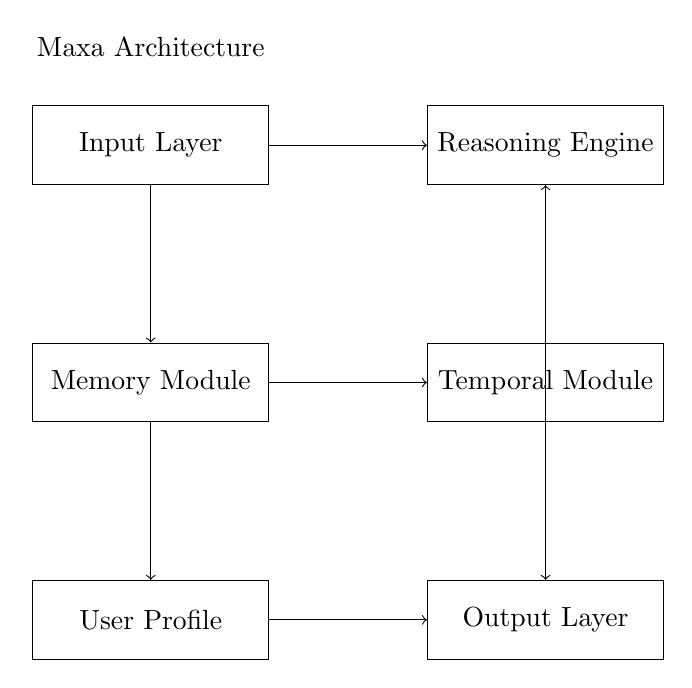
\begin{tikzpicture}[node distance=2cm, auto]
    % Nodes
    \node[draw, rectangle, minimum width=3cm, minimum height=1cm] (input) {Input Layer};
    \node[draw, rectangle, minimum width=3cm, minimum height=1cm, below=of input] (memory) {Memory Module};
    \node[draw, rectangle, minimum width=3cm, minimum height=1cm, right=of input] (reasoning) {Reasoning Engine};
    \node[draw, rectangle, minimum width=3cm, minimum height=1cm, right=of memory] (temporal) {Temporal Module};
    \node[draw, rectangle, minimum width=3cm, minimum height=1cm, below=of memory] (profile) {User Profile};
    \node[draw, rectangle, minimum width=3cm, minimum height=1cm, right=of profile] (output) {Output Layer};

    % Arrows
    \draw[->] (input) -- (reasoning);
    \draw[->] (input) -- (memory);
    \draw[->] (memory) -- (temporal);
    \draw[->] (memory) -- (profile);
    \draw[->] (profile) -- (output);
    \draw[->] (temporal) -- (reasoning);
    \draw[->] (reasoning) -- (output);

    % Legend
    \node[above=0.5cm of input, align=center] {Maxa Architecture};
\end{tikzpicture}
\end{document}
